%%%%%%%%%%%%%%%%%%%%%%%%%%%%%%%%%%%%%%%%%

%----------------------------------------------------------------------------------------
%	PACKAGES AND OTHER DOCUMENT CONFIGURATIONS
%----------------------------------------------------------------------------------------

\documentclass{article}

\input{C:/Code/TexStudio/templates/structure.tex} % Include the file specifying the document structure and custom commands

%----------------------------------------------------------------------------------------
%	ASSIGNMENT INFORMATION
%----------------------------------------------------------------------------------------

\title{Assignment \#4} % Title of the assignment

\author{Name:Cao Mingming \indent \indent ID:2018311770\\ \texttt{cmm18@mails.tsinghua.edu.cn}} % Author name and email address

\date{Tsinghua University --- \today} % University, school and/or department name(s) and a date

%----------------------------------------------------------------------------------------

\begin{document}

\maketitle % Print the title

%----------------------------------------------------------------------------------------
%	INTRODUCTION
%----------------------------------------------------------------------------------------

\section{Problem 1} % Unnumbered section
Draw the curves similar to Fig. 2.4 for the range of $0<d<2R$ with the parameters that you are
interested in e.g. $R = 15 cm$, $\lambda= 0.37 \mu m$ or $R = 20 cm, \lambda = 0.78\mu $m or $ R=10cm, \lambda=0.532 \mu m$.
\section*{Solution}
According to eqaution 2.21 and 2.22 in textbook we know that,
\begin{equation}
	\begin{array}{l}
		\omega^2=\left(\frac{\lambda R}{n\pi}\right)\sqrt{\frac{d}{2R-d}}\\
		\\
		\omega_{0}^2=\left(\frac{\lambda}{n\pi}\right)\sqrt{\frac{dR}{2}-\frac{d^2}{4}}
	\end{array}
\end{equation}
Choose the parameters as $R = 20 cm, \lambda = 0.78\mu $,we can get the following figure.
\begin{figure}[h]
	\centering
	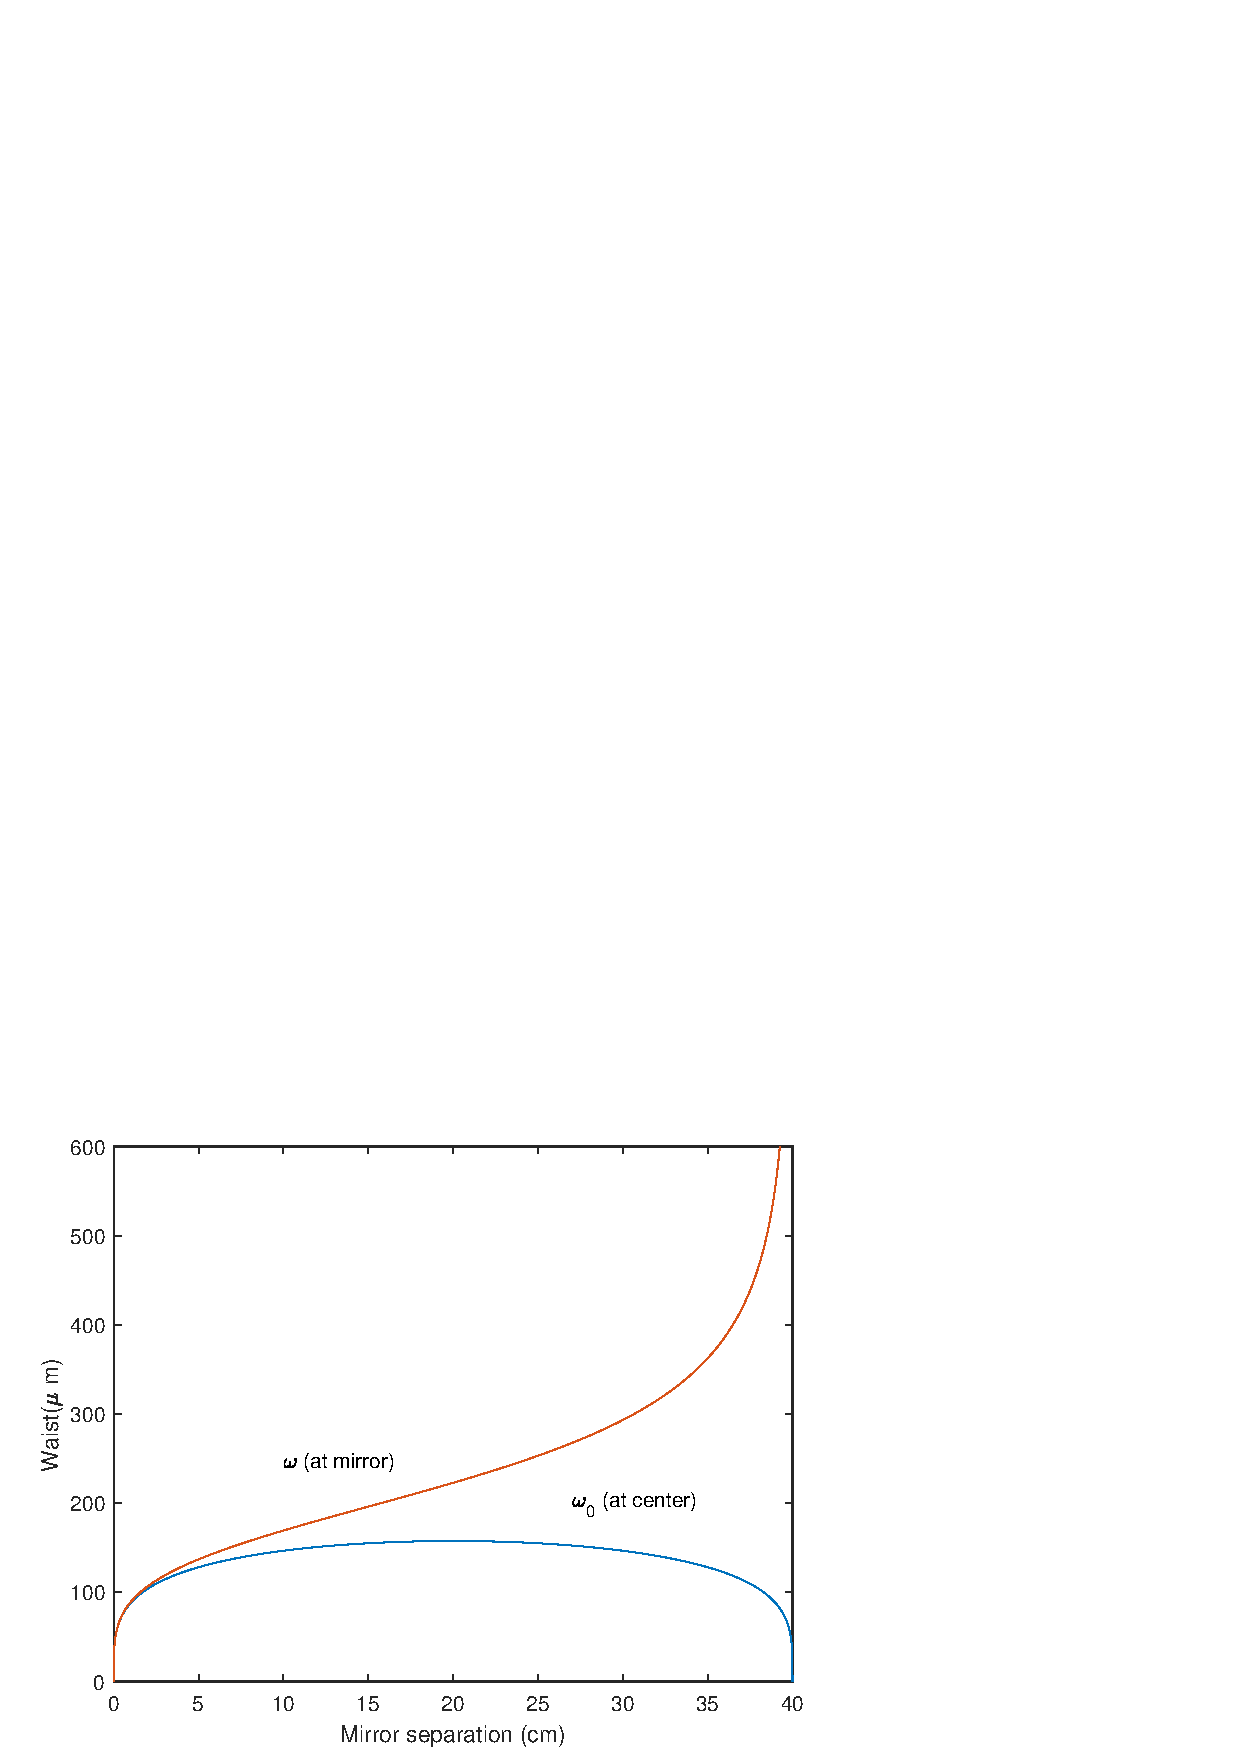
\includegraphics[width=10cm]{f1.pdf}
	\caption{Figure of $\omega $}
\end{figure}

\section{Problem 2}
(a) Find the stability condition in terms of $d_3 , d_1+2d_2$ , and $R$.
(b) Find the small waist within $d_3$ range and the large waist within $d_1$ in terms of $g_1$ ($=1-(d_1+2d_2 )/R$), $g_2$($=1-d_3/R$) and $R$.

\begin{figure}[ht]
	\centering
	\includegraphics[width=10cm]{f2.png}
	\caption{Optical cavity}
\end{figure}

\section*{Solution}
According to figure 2 we could get the ABCD matrix as,
\begin{equation}
	\begin{aligned}
	\begin{pmatrix}
	A & B\\
	C & D 
	\end{pmatrix}
	&=\begin{pmatrix}
	1 & 0\\
	-\frac{2}{R} & 1
	\end{pmatrix}
	\begin{pmatrix}
	1 & d_1+2d_2\\
	0 & 1
	\end{pmatrix}
	\begin{pmatrix}
	1 & 0\\
	-\frac{2}{R} & 1
	\end{pmatrix}
	\begin{pmatrix}
	1 & d_3\\
	0 & 1
	\end{pmatrix}\\
	\\
	&=\begin{pmatrix}
	2g_1-1 & R(g_1+g_2-2g_1g_2)\\
	-\frac{4g_1}{R} & 4g_1g_2-2g_1-1
	\end{pmatrix}
	\end{aligned}
\end{equation}
where 
\begin{equation}
\begin{array}{l}
g_1=1-\frac{d_1+2d_2}{R}\\
\\
g_2=1-\frac{d_3}{R}
\end{array}
\end{equation}
It is the same as what have sloved in two mirror situation  which means we could get the stablity condition as,
\begin{equation}
|A+D|\leq2\Rightarrow|4g_1g_2-2|\leq2\Rightarrow|0\leq g_1g_2\leq 1
\end{equation}


\end{document}